\documentclass[letterpaper,journal]{IEEEtran}
\usepackage{amsmath,amssymb,amsfonts}
\usepackage{booktabs}
\usepackage{graphicx}
\usepackage{cite}
\usepackage{url}
\usepackage[hidelinks]{hyperref}
\usepackage{xcolor}

\newcommand{\E}{\mathbb E}
\newcommand{\Prb}{\mathbb P}
\newcommand{\Var}{\operatorname{Var}}
\newcommand{\Cov}{\operatorname{Cov}}
\newcommand{\Tr}{\operatorname{Tr}}
\newcommand{\TV}{\operatorname{TV}}
\newcommand{\cF}{\mathcal F}
\newcommand{\cH}{\mathcal H}
\newcommand{\one}{\mathbf 1}
\newcommand{\AOC}{\textsc{AOC}}
\newcommand{\vAOC}{\textsc{vAOC}}
\newcommand{\TBD}[1]{\textcolor{red}{[\textbf{LOCKED RESULT PENDING
AUDIT:} #1]}}
\newcommand{\TBDSequential}{\TBD{sequential endpoint}}
\newcommand{\TBDOffline}{\TBD{offline endpoint}}

\begin{document}

\title{What Syndrome Data Can and Cannot Detect:
Accessible-Observable Sequential Change Detection for
Topological Quantum Error Correction}

\author{Rongzhou (Lachlan) Chen%
\thanks{Run 5 working paper. Exact statements, controlled-model results,
circuit-level results, and unrun or unaudited endpoints are labeled
separately. The sequential and offline locked-result fields in this staged
draft are explicit placeholders and support no present advantage claim.}}

\maketitle

\begin{abstract}
Surface-code monitors often compress a detector stream to a defect rate,
although drift can preserve every detector marginal and the complete count
distribution while changing spatial or temporal correlations. We formulate
the resulting limitation at the process level: if two hypotheses induce the
same law on the entire accessible observation path, every stopping rule
adapted to that path has the same distribution under both hypotheses.
One-round equality alone is insufficient when dependence changes. We then
construct a periodic two-endpoint detector model in which (i) spatial
chain-length drift is exactly count-blind but is identified by two signed
translation correlations, (ii) temporal persistence preserves the complete
one-cycle syndrome law but changes adjacent-pair likelihoods, and (iii) a
closed logical cycle is pathwise syndrome-invisible. The spatial likelihood
reduces exactly to three translation statistics, and the temporal pair
likelihood has a closed form. A predictable, bounded observable score is
embedded in the established Shiryaev--Roberts/e-detector construction; under
an exact null it has an average-run-length guarantee. Locked identity checks
give zero count total variation and numerical likelihood errors below
$9\times10^{-15}$. Separate audits find a $4.20$--$4.23$ copy-RMSE penalty
for local-Pauli shadows versus native all-$Z$ readout on declared $ZZ$
observables, and a controlled Stim/PyMatching experiment reduces the
distance-seven correlated-regime logical-error rate from $0.01526$ to
$0.01120$ when the injected post-change correlation model is known.
That circuit result tests decoder utility, not change detection. The
preregistered sequential and offline endpoints remain withheld in this staged
draft pending their locked audits; consequently no algorithmic-advantage
claim is made here.
\end{abstract}

\begin{IEEEkeywords}
accessible observables, change detection, e-detectors, quantum error
correction, surface code, syndrome correlations
\end{IEEEkeywords}

\section{Introduction}

\IEEEPARstart{S}{urface-code} syndrome data are valuable not only for
decoding but also for estimating and tracking noise. Existing work learns
detector-error-model (DEM) events from repeated syndromes, performs Bayesian
noise inference, and adapts decoding graphs under drift and correlated
faults~\cite{wang2023dgr,blumekohout2025,takou2026,kobori2025}. The first
question is therefore not whether syndromes can reveal drift in general. It
is which drift remains identifiable after a declared compression, locality
restriction, measurement policy, and history budget.

Run 4 of the accompanying repository gave an exact static example: a
sub-distance observer is blind to a toric-code flux sector, whereas a
noncontractible Wilson loop resolves it. That local blindness and the logical
role of closed chains are established topological-code/QEC
structure~\cite{kitaev2003,dennis2002,knill1997,bravyi2010}; ribbon-operator
discovery is also prior art~\cite{bridgeman2016}. Run 5 moves from static
sector classification to a practical sequential question: can correlation
drift be detected at fixed syndrome and false-alarm budgets when rate/count
statistics are provably blind?

The paper makes four bounded contributions.
\begin{enumerate}
\item It states an accessible-\emph{process} no-go certificate. Equality of
the full accessible path laws, not merely one-round marginals, is the
condition for sequential impossibility.
\item It gives exact controlled spatial, temporal, and logical separations.
For the spatial family, the complete count process is invariant while
$(\bar z,g_1,g_2)$ is sufficient; for the temporal family, one-cycle laws
are equal while adjacent-pair laws differ.
\item It places predictable raw and variance-aware observable contrasts in an
established bounded e-factor/Shiryaev--Roberts construction, clearly
separating one-shot mean-gap, variance-sensitive, and likelihood-growth
objectives.
\item It reports locked identifiability, measurement-policy, and
circuit-level decoder-utility audits. The primary locked sequential and
offline diagnostic conclusions are intentionally not filled in until their
outputs pass the declared audit.
\end{enumerate}

This is neither a claim of the first QEC drift detector nor a new covariance
test. Page's CUSUM, Hotelling whitening, Kelly log growth, and e-detectors are
foundations~\cite{page1954,hotelling1931,kelly1956,shin2024}. Classical
shadows and shadow-based sequential quantum change detection are also
established~\cite{huang2020,zecchin2026}. The contribution is a reproducible
information-access hierarchy with negative certificates, matched witnesses,
and explicit evidence boundaries.

\section{Prior Art and Evidence Boundary}

\subsection{Restricted information and sequential detection}

Helstrom theory is the unrestricted binary quantum-measurement ceiling for
fixed states, priors, and loss~\cite{helstrom1976}. Restricted measurement
families induce different distinguishability norms~\cite{matthews2009}, and
group-symmetric quantum hypothesis testing is established~\cite{hiai2009}.
Most Run 5 experiments begin \emph{after} stabilizer measurement and receive a
classical syndrome stream. Helstrom is therefore a conceptual upstream
ceiling, not an implemented baseline for every experiment.

The variance-aware direction $V^{-1}\delta$ is classical
Fisher/Hotelling geometry, not an \AOC\ invention~\cite{hotelling1931}. Its
unrestricted quantum tangent-space analogue is tied to symmetric logarithmic
derivatives and quantum Fisher information~\cite{braunstein1994}. Likewise,
the average-run-length result below specializes the e-detector framework of
Shin, Ramdas, and Rinaldo~\cite{shin2024}; it is not a new general
sequential-testing theorem.

\subsection{Four evidence levels}

Table~\ref{tab:evidence} fixes the vocabulary used throughout. ``Exact''
means exact under stated mathematical assumptions, not physically complete.
The controlled finite-mixture model omits coherent faults, leakage, device
scheduling, and many calibration mechanisms. Stim samples are circuit-level
stabilizer simulations~\cite{gidney2021}, and PyMatching is an established
MWPM decoder~\cite{higgott2022,higgott2025}. Neither package turns simulated
data into hardware evidence.

\begin{table}[t]
\centering
\caption{Evidence levels and permitted conclusions.}
\label{tab:evidence}
\begin{tabular}{@{}p{0.22\columnwidth}p{0.69\columnwidth}@{}}
\toprule
Level & Meaning in this paper\\
\midrule
Exact statement & Proof under the displayed probability/QEC model.\\
Controlled model & Exact likelihood or Monte Carlo from the declared
phenomenological family.\\
Circuit level & Stim/DEM samples and PyMatching for the specified simulated
circuit and injected channel.\\
Hardware & Physical-device samples; none are used in Run 5.\\
\bottomrule
\end{tabular}
\end{table}

\section{Accessible-Process Theory}

\subsection{The correct sequential no-go statement}

Let $Y=(Y_1,Y_2,\ldots)$ be the full observation stream. An access policy
$\cH$ maps it to $Z=\cH(Y)$; this map may retain per-round counts, a finite
history, local correlation features, or a separately costed audit. Denote the
path laws by $P_j^Z=\cH_\#P_j$, $j\in\{0,1\}$.

\textbf{Theorem 1 (accessible-process no-go).}
If $P_0^Z=P_1^Z$, then every randomized stopping rule adapted only to the
accessible filtration has the same stopping-time law under $P_0$ and $P_1$.
In particular, for every horizon $T$,
\begin{equation}
P_1(\tau\leq T)=P_0(\tau\leq T).
\label{eq:path-nogo}
\end{equation}

\begin{IEEEproof}
Let $U$ be the detector's data-independent random seed. Any such stopping
rule is a measurable function $\tau=\phi(Z,U)$. The assumption implies
$P_0^Z\otimes P^U=P_1^Z\otimes P^U$. Applying the measurable map $\phi$ to
both sides gives equality of the stopping-time pushforwards and hence
\eqref{eq:path-nogo}.
\end{IEEEproof}

\textbf{Corollary 1 (iid compression).}
Suppose $Z_t=h(Y_t)$ and the accessible rounds are iid under each hypothesis.
If $h_\#P_0^{(1)}=h_\#P_1^{(1)}$, their path laws are equal and
Theorem~1 applies.

\begin{IEEEproof}
The two accessible path measures are products of the same one-round
pushforward.
\end{IEEEproof}

The iid condition is essential. The temporal experiment below deliberately
keeps the complete one-cycle law fixed while changing persistence. A
history-aware detector then has power because the accessible \emph{path}
laws are not equal. Any statement that infers sequential blindness from
one-round marginal equality alone would be false.

Data processing provides the quantitative companion
\begin{equation}
\TV(\cH_\#P_0,\cH_\#P_1)\leq \TV(P_0,P_1).
\label{eq:data-processing}
\end{equation}
Thus enriching the accessible algebra or history can reveal information that
compression erased, but post-processing a fixed accessible stream cannot
recreate it.

\subsection{Logical-cycle pathwise certificate}

For a chain complex with syndrome boundary map $\partial$, add a closed chain
$c\in\ker\partial$ to an error chain $E$. Then
\begin{equation}
\partial(E+c)=\partial E.
\label{eq:logical-nogo}
\end{equation}
A coupling that applies the same modification to each selected path therefore
gives identical complete syndrome histories, while a homologically
nontrivial $c$ can flip a logical/Wilson audit. This is an executable instance
of known QEC/local-topological-order structure, not a new toric-code or Wilson
theorem. Gauge-region algebras can also have nontrivial centers and need not
factor naively~\cite{casini2014}, so future gauge applications must state the
accessible algebra rather than assume a tensor-product region.

\section{Exact Controlled Detector Model}

\subsection{Spatial correlation drift}

Consider an $L\times L$ periodic check lattice with $m=L^2$ detectors. In one
round, $J\sim\operatorname{Bernoulli}(\eta)$. If $J=0$, the clean syndrome is
zero. If $J=1$, choose a uniformly translated and oriented straight chain
with length $\ell=1$ with probability $1-q$ and $\ell=2$ with probability
$q$, and set its two endpoints to one. Finally, pass every detector through an
independent binary symmetric channel (BSC) with crossover $\epsilon$.

For every detector $i$,
\begin{equation}
\Prb_q(Y_i=1)=\epsilon+(1-2\epsilon)\frac{2\eta}{m},
\label{eq:marginal}
\end{equation}
which is independent of $q$. More strongly, conditional on $J=1$ every clean
template has Hamming weight two. Since iid BSC noise is invariant under
coordinate permutations, the complete distribution of
$C=\sum_iY_i$ is independent of chain length and hence of $q$. Independent
rounds therefore give an exact count-\emph{process} no-go by Corollary~1,
not merely a zero mean-gap observation.

Let $z_i=1-2y_i$, $\bar z=m^{-1}\sum_i z_i$, and
\begin{equation}
g_\ell(y)=\frac{1}{2m}\sum_{v,o\in\{x,y\}}
z_vz_{v+\ell e_o}.
\label{eq:gell}
\end{equation}
Write $B_0(y)$ for the BSC probability given the all-zero clean template and
$r=(1-\epsilon)/\epsilon$. Define
$a=(r+r^{-1})/2$ and $b=(r-r^{-1})/2$. Averaging a two-endpoint likelihood
ratio over translations and orientations gives
\begin{equation}
K_\ell(y)=a^2-2ab\,\bar z+b^2g_\ell(y).
\label{eq:kell}
\end{equation}
The exact one-round likelihood is therefore
\begin{equation}
P_q(y)=B_0(y)\left[(1-\eta)+
\eta\{(1-q)K_1(y)+qK_2(y)\}\right].
\label{eq:spatial-likelihood}
\end{equation}

\textbf{Theorem 2 (translation sufficiency and signed gap).}
In the declared spatial family, $(\bar z,g_1,g_2)$ is sufficient for $q$.
Moreover, for two parameters $q_0,q_1$,
\begin{equation}
\begin{split}
&\left(\E_{q_1}g_1-\E_{q_0}g_1,\,
\E_{q_1}g_2-\E_{q_0}g_2\right)\\
&\qquad =
\frac{2\eta(1-2\epsilon)^2}{m}(q_1-q_0)(-1,+1).
\end{split}
\label{eq:pair-gap}
\end{equation}

\begin{IEEEproof}
Equation~\eqref{eq:spatial-likelihood} follows by writing the likelihood ratio
for endpoints $u,v$ as
$(a-bz_u)(a-bz_v)$ and averaging. Its dependence on $q$ is entirely through
$(\bar z,g_1,g_2)$, proving sufficiency by factorization. For
\eqref{eq:pair-gap}, independent readout flips multiply every clean
two-point spin product by $(1-2\epsilon)^2$. Moving event mass
$\eta(q_1-q_0)$ from length one to length two decreases the matching
length-one average and increases the matching length-two average; uniform
translation/orientation supplies the factor $2/m$.
\end{IEEEproof}

This sufficiency is model-specific. It does not say that three statistics are
sufficient for a general surface-code circuit, arbitrary DEM, or hardware
noise.

\subsection{Temporal persistence drift}

Let $H_t\in\{0,1\}$ denote the chain-length state, with stationary
$\Prb(H_t=1)=q_0$, and define
\begin{equation}
X_t=\frac{H_t-q_0}{\sqrt{q_0(1-q_0)}}.
\end{equation}
The null uses iid $H_t$. Under the alternative,
\begin{equation}
\Prb(H_{t+1}=1\mid H_t)=q_0+\kappa(H_t-q_0),
\label{eq:markov}
\end{equation}
so the stationary one-cycle law is unchanged and
$\E(X_tX_{t+1})=\kappa$. Let $e_h(y)$ be the emission density at state $h$,
$p_0(y)=\sum_h\pi_he_h(y)$, and
\begin{equation}
a(y)=\E_0[X_t\mid Y_t=y].
\end{equation}

\textbf{Theorem 3 (exact adjacent-pair likelihood ratio).}
For a stationary adjacent pair under \eqref{eq:markov}, relative to two iid
null cycles,
\begin{equation}
L_\kappa(y,y')=1+\kappa a(y)a(y'),\qquad
\E_0 L_\kappa=1.
\label{eq:pair-lr}
\end{equation}

\begin{IEEEproof}
For a binary stationary state, the joint state mass can be written
$\pi_h\pi_{h'}[1+\kappa x_hx_{h'}]$, where $x_h$ is the standardized state
value. Multiplying by $e_h(y)e_{h'}(y')$, summing over $h,h'$, and dividing by
$p_0(y)p_0(y')$ gives \eqref{eq:pair-lr}. Null expectation one follows by
integrating the likelihood ratio, equivalently from $\E_0a(Y)=0$.
\end{IEEEproof}

Nonoverlapping pairs give independent null e-factors and a deliberately
pair-restricted alternative. They discard cross-block alternative
correlations. A forward-filter HMM is retained as a model-aware ceiling, not
misnamed as the same pair likelihood.

\section{Predictable Observable e-Detector}

\subsection{Raw and variance-aware directions}

Encode one syndrome round as the trace-one correlation state
\begin{equation}
R_t=\frac{z_tz_t^\top}{m}.
\label{eq:correlation-state}
\end{equation}
A raw \AOC\ witness is the positive support of a projected difference between
a past-only live estimate and the null state. Translation averaging reduces
it to displacement or Fourier features. This raw direction targets a bounded
one-shot expectation gap, analogous to restricted total-variation
discrimination. It is not a quickest-change solution.

For an accessible feature vector $G_t=g(R_t)$ with exact null mean $\mu_0$
and covariance $V_0$, a predictable live estimate gives
\begin{equation}
\widehat\delta_{t-1}=\widehat\E_{t-1}G-\mu_0,\qquad
w_{t-1}=(V_0+\lambda I)^{-1}\widehat\delta_{t-1}.
\label{eq:whitened}
\end{equation}
This is regularized Hotelling/Fisher whitening. Locally, it is the
least-squares projection of a likelihood score onto the accessible feature
span. We call the resulting restricted implementation \vAOC\ only to identify
its provenance in this repository, not to claim new whitening mathematics.

Let $B(w)$ be a predictable deterministic bound satisfying
$|w^\top(G_t-\mu_0)|\leq B(w)$ for every possible $G_t$, and set
\begin{equation}
s_t=\frac{w_{t-1}^\top(G_t-\mu_0)}{B(w_{t-1})}\in[-1,1].
\label{eq:bounded-score}
\end{equation}
When $B=0$, set $s_t=0$. For predictable $\beta\in[0,1]$,
\begin{equation}
L_t(\beta)=1+\beta s_t\geq0,\qquad
\E_0[L_t(\beta)\mid\cF_{t-1}]=1.
\label{eq:e-factor}
\end{equation}

\subsection{Shiryaev--Roberts recursion and guarantee}

For a fixed grid $\mathcal B$, initialize $S_0^\beta=0$ and update
\begin{equation}
S_t^\beta=(S_{t-1}^\beta+1)L_t(\beta),\quad
\bar S_t=|\mathcal B|^{-1}\sum_{\beta\in\mathcal B}S_t^\beta.
\label{eq:sr}
\end{equation}
Stop at $\tau_\gamma=\inf\{t:\bar S_t\geq\gamma\}$.

\textbf{Proposition 1 (exact-null average run length).}
Under \eqref{eq:e-factor} and standard integrability conditions,
\begin{equation}
\E_0\tau_\gamma\geq\gamma.
\label{eq:arl}
\end{equation}

\begin{IEEEproof}
For each $\beta$,
$S_t^\beta-t$ is a null martingale because
$\E_0(S_t^\beta\mid\cF_{t-1})=S_{t-1}^\beta+1$. The mixture has the same
property. Optional stopping at $\tau_\gamma\wedge n$ gives
$\E_0(\tau_\gamma\wedge n)=
\E_0\bar S_{\tau_\gamma\wedge n}\geq
\gamma\Prb_0(\tau_\gamma\leq n)$.
If the stopping time is defective, its extended expectation is infinite;
otherwise monotone convergence yields \eqref{eq:arl}. This is the
Shiryaev--Roberts/e-detector argument~\cite{shin2024}.
\end{IEEEproof}

The statistic $\bar S_t$ is an e-\emph{detector}, not a unit-mean e-process:
under the null its expectation grows as $t$. Equation~\eqref{eq:arl} is an
average-run-length guarantee, not a Ville bound on the probability of ever
crossing $\gamma$. If the witness or tuning uses current/future test data, or
if centering/bounds are invalid, \eqref{eq:e-factor} need not hold. Here
$\mu_0$ is analytic. Conditional on independent auxiliary data, covariance,
ridge, and logistic-direction fitting only fix a bounded, predictable effect,
so exact-null centering preserves \eqref{eq:e-factor}. Estimating the null mean
itself from finite data without uncertainty protection does not automatically
preserve the guarantee.

\begin{figure}[t]
\centering
\fbox{\begin{minipage}{0.92\columnwidth}
\textbf{Algorithm 1: Predictable accessible-observable e-detector}\\[2pt]
\textbf{Input:} exact or uncertainty-valid $\mu_0$; independently fitted $V_0$;
feature
bank $g$; predictable live-state rule; ridge $\lambda$; betting grid
$\mathcal B$; threshold $\gamma$.\\
\textbf{Initialize:} past-only estimator and $S_0^\beta=0$ for every
$\beta\in\mathcal B$.\\
\textbf{For} $t=1,2,\ldots$:\\
\quad 1) Before seeing $Y_t$, form the raw support direction or
\eqref{eq:whitened} from $\cF_{t-1}$.\\
\quad 2) Observe $Y_t$, compute $G_t=g(R_t)$, and normalize by a declared
support bound to obtain \eqref{eq:bounded-score}.\\
\quad 3) Update every component by \eqref{eq:sr}; alarm if
$\bar S_t\geq\gamma$.\\
\quad 4) If no alarm occurs, update the live estimate using $Y_t$.\\
\textbf{Output:} stopping time, predictable witness history, and
component evidence.
\end{minipage}}
\caption{The witness must be frozen before the current observation. Independent
calibration and held-out tuning are part of the data budget.}
\label{alg:detector}
\end{figure}

\subsection{A necessary restart-at-change correction}

If a control is exactly blind, then $s_t=0$, $L_t=1$, and
$S_t=t$. With threshold $\gamma$ and changepoint $\nu<\gamma$, the naive
quantity $\gamma-\nu$ would falsely credit the age of the SR clock as
post-change evidence. The protocol was therefore amended after a reduced
pilot and before the locked run:
\begin{enumerate}
\item the primary response restarts every method at the changepoint and
measures restricted mean delay on the same post-change segment;
\item each restart delay is compared with same-horizon no-change restricted
run length;
\item surveillance results separately report pre-change alarms and condition
post-change delay on $\tau>\nu$; and
\item independent no-change streams remain the ARL/censoring audit.
\end{enumerate}
This amendment prevents deterministic clock accumulation from masquerading
as detection.

\section{Locked Design and Named-Comparator Criterion}

The primary controlled model uses $L=5$, $\eta=0.65$,
$\epsilon=0.03$, and $q_0=0.35$. Spatial alternatives are
$q_1\in\{0.45,0.55,0.65\}$; temporal alternatives are
$\kappa\in\{0.50,0.75,0.90\}$. Locked-test comparisons use identical paired
streams, changepoints, physical-cycle horizons, and seeds. Calibration uses
4096 physical cycles per family. A spatial update costs one cycle and uses
threshold 1000; a temporal pair update costs two cycles and uses threshold
500. Both target an average run length of at least 1000 physical cycles.

The named non-oracle comparator is a linear logistic direction on the same
Fourier simplex/pair-simplex, affinely mapped into $[0,1]$, centered at the
analytic null, and passed through the same bounded-score SR. It was chosen
after the independent offline audit but before the sequential locked test; it
is not claimed to be the strongest generic baseline. Its training uses eight
independent streams per class and 512 cycles per stream. \vAOC\ receives the
same $8\times512=4096$ alternative ridge-validation cycles plus 4096 null
covariance-calibration cycles; the logistic comparator receives 4096 cycles
from each class with the same stream structure.

The comparison set includes a provably blind detector-count control,
mean-vector scans, matched signed displacement correlation, shrinkage
Hotelling/covariance and spectral tests, RBF-Hamming MMD, raw \AOC,
\vAOC, the named logistic comparator, direct observable-bank e-detectors,
exact grid likelihood-ratio SR, and a known-post/HMM ceiling. Separate
logistic-regression and RBF-SVM window classifiers are offline diagnostics
without sequential guarantees.

At $q_1=0.55$ and $\kappa=0.75$, let
$D_i=T_i^{\vAOC}-T_i^{\rm logit}$. Restricted delays lie in $[0,H]$, hence
independent paired differences lie in $[-H,H]$. Under
$H_0:\E D_i\geq0$, the distribution-free one-sided Hoeffding p-value and
Bonferroni simultaneous upper bound are
\begin{align}
p_{\rm H}
&=\min\!\left\{1,\exp\!\left[
-\frac{n\max(0,-\bar D)^2}{2H^2}\right]\right\},\\
U_{\rm H}
&=\bar D+H\sqrt{\frac{2\log(m/\alpha)}{n}},\qquad m=2.
\label{eq:named-comparison}
\end{align}
Holm adjustment is applied to the two p-values. A paired percentile-bootstrap
interval is descriptive only. For each task, $U_{\rm H}<0$, the
Holm-adjusted p-value must be below 0.05, and the ARL condition must hold; the
repo-level flag additionally requires both tasks to pass. Thus the tested
contrast is
\begin{equation}
\operatorname{RMDD}_{\vAOC}
-\operatorname{RMDD}_{\mathrm{named\ logistic\ comparator}}.
\label{eq:comparison-estimand}
\end{equation}
Even a pass supports only \vAOC\ versus this named comparator on these two
controlled tasks, not strongest-baseline or general algorithmic superiority.
Exact likelihoods and full-HMM/known-post procedures are ceilings, not
targets to beat. Failure is an informative negative result and does not alter
the no-go theorems.

\section{Locked Results Available in This Draft}

\subsection{Exact identifiability certificates}

The locked controlled audit used $L=5$, $q_0=0.35$, $q_1=0.55$,
$\eta=0.65$, and $\epsilon=0.03$. Table~\ref{tab:identities} separates exact
identity residuals from finite-sample discrimination summaries. The spatial
AUC used $200{,}000$ samples per regime; the temporal AUC used $100{,}000$
pairs per regime. The AUCs are not claims of strong practical performance;
they verify that the richer observable contains nonzero information where
the declared lower level is exactly blind.

\begin{table}[t]
\centering
\caption{Controlled identifiability audit.}
\label{tab:identities}
\begin{tabular}{lr}
\toprule
Quantity & Locked value\\
\midrule
Complete count-PMF total variation & $0$\\
Maximum detector-marginal gap & $0$\\
Spatial sufficient/direct log-LR error & $5.55\times10^{-15}$\\
Temporal pair closed-form/direct error & $8.91\times10^{-15}$\\
Spatial exact-likelihood ROC AUC & $0.573775$\\
Temporal pair-likelihood ROC AUC & $0.576994$\\
Logical syndrome-history total variation & $0$\\
Syndrome-only / logical-audit success & $0.5/1.0$\\
\bottomrule
\end{tabular}
\end{table}

\begin{figure}[t]
\centering
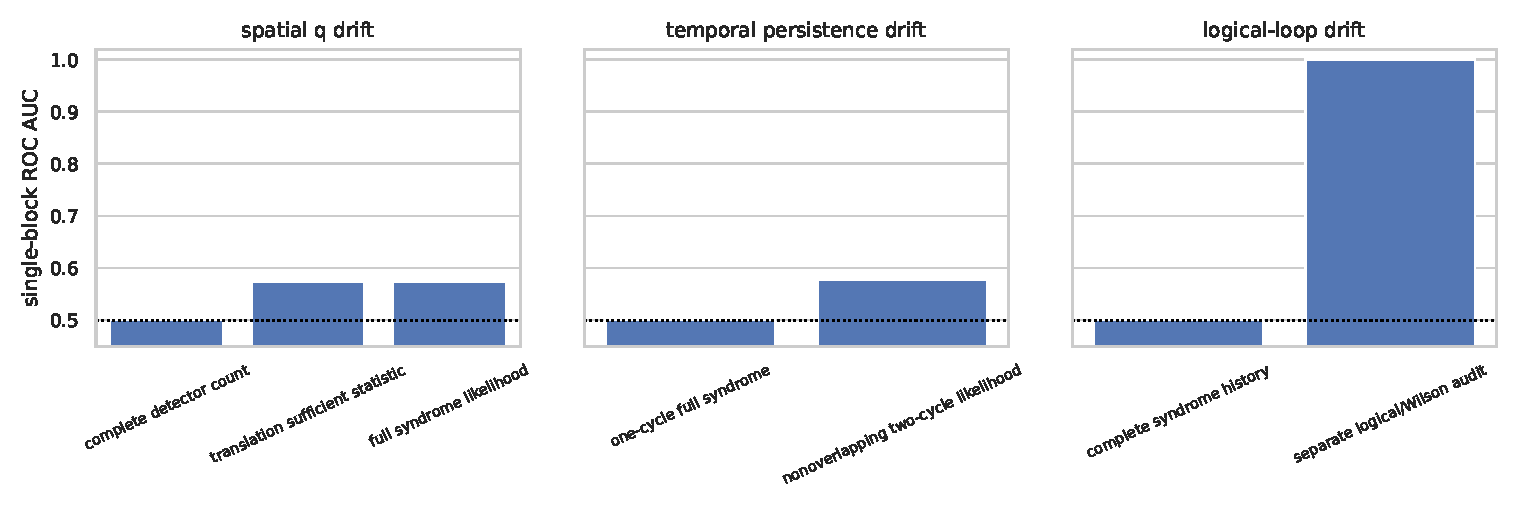
\includegraphics[width=\columnwidth]{../../experiments/run5/results/identifiability/accessibility_hierarchy.pdf}
\caption{Locked controlled-model access hierarchy. Count blindness is exact
for the spatial iid family; one-cycle equality in the temporal family does
not imply path blindness. The logical loop is syndrome-invisible and requires
a separately costed logical audit.}
\label{fig:hierarchy}
\end{figure}

\subsection{Measurement-policy audit}

For 100 declared $ZZ$ displacement observables on the $L=5$ diagonal
controlled states, the local-Pauli shadow estimator is
\begin{equation}
\widehat{\langle Z_iZ_j\rangle}
=9\,\one\{B_i=B_j=Z\}\,b_ib_j.
\label{eq:shadow}
\end{equation}
Only $1/9$ of copies contribute to a given pair, whereas native all-$Z$
readout contributes every copy. Across 256 repetitions at 4096 copies, the
mean RMSEs were $0.045054$ (shadow) versus $0.010737$ (native) at
$q=0.35$, and $0.045192$ versus $0.010674$ at $q=0.65$. The ratios are
$4.20$ and $4.23$.

\begin{figure}[t]
\centering
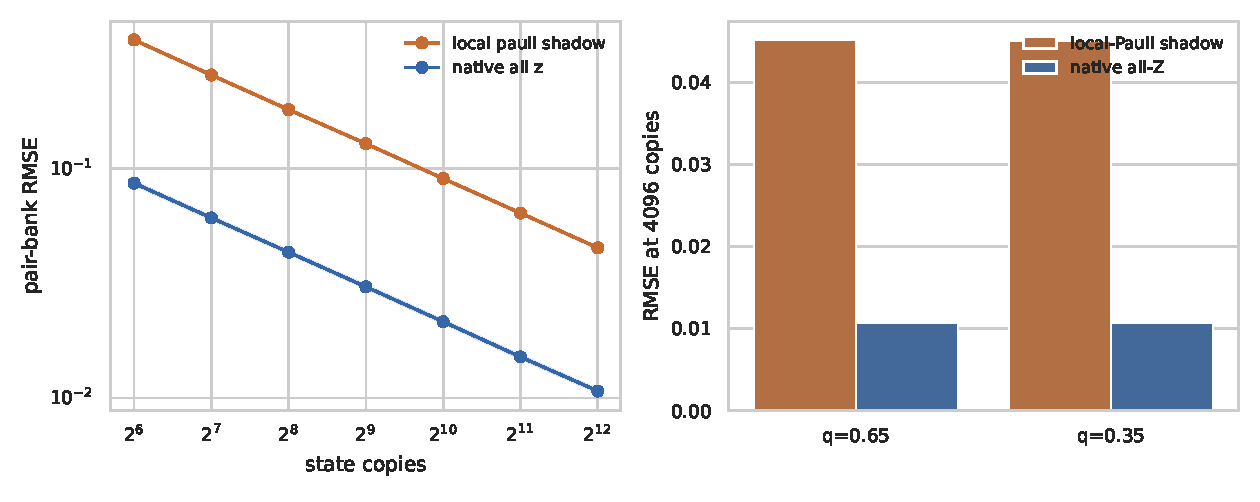
\includegraphics[width=\columnwidth]{../../experiments/run5/results/shadow_measurement/shadow_measurement_audit.pdf}
\caption{Locked measurement-policy audit. Native all-$Z$ is matched to the
declared diagonal $ZZ$ bank; the shadow penalty measures universality cost.
This is not an implementation of eSCD and does not establish superiority to
classical-shadow sequential detection.}
\label{fig:shadow}
\end{figure}

\subsection{Circuit-level decoder utility}

A separate locked circuit experiment generated
\texttt{surface\_code:rotated\_memory\_z} circuits at distances
$d\in\{3,5,7\}$ with rounds equal to distance, using Stim 1.16.0 and
PyMatching 2.4.0. Each reference/correlated regime used $200{,}000$ shots per
distance. The circuit noise parameters were post-Clifford depolarization
$0.001$, measurement/reset flips $0.002$, marginal data-$X$ probability
$0.02$, and common paired data-$X$ probability $0.01$. An exact DEM audit
found a maximum reference--correlated detector-marginal gap
$3.33\times10^{-16}$, below the declared $10^{-12}$ tolerance.

At the predeclared distance-seven correlated endpoint, the static,
ordinary-post, and correlation-aware logical-error rates were $0.01653$,
$0.01526$, and $0.01120$. The paired difference between ordinary-post and
correlation-aware decoding was $0.00406$, with paired-bootstrap 95\% interval
$[0.00369,0.004435]$, a 26.6\% relative reduction. Under the reference
regime, however, the same three rates were $0.019785$, $0.021605$, and
$0.022175$: applying the correlation-aware model when it is wrong degrades
performance.

\begin{figure}[t]
\centering
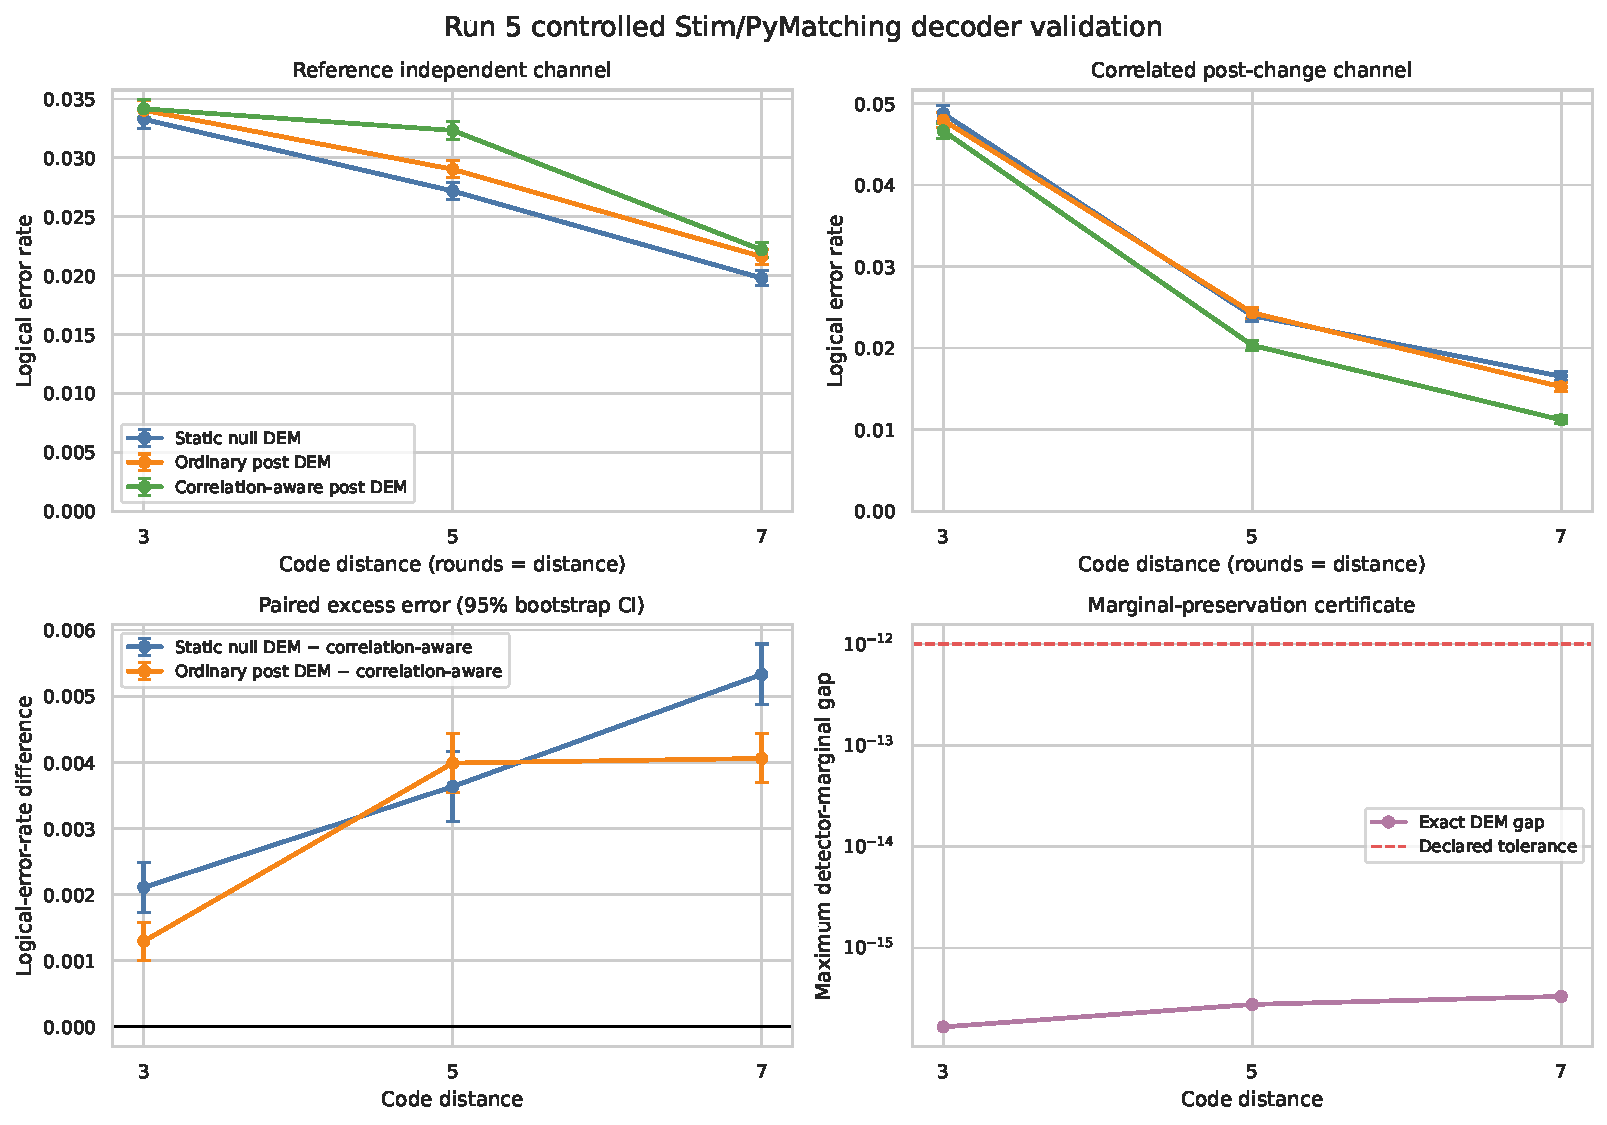
\includegraphics[width=\columnwidth]{../../experiments/run5/results/circuit_level_locked/decoder_validation.pdf}
\caption{Locked Stim/PyMatching circuit-level simulation. Correlation-aware
decoding helps only in the injected correlated regime and is harmful under
the reference regime, motivating reliable model selection. The injected
channel and decoder models are known; no online detector is tested here.}
\label{fig:decoder}
\end{figure}

This result supports downstream utility of correct correlation modeling under
the specified simulator. It does not show that \AOC/\vAOC\ detects the
change, does not compare a full DGR reproduction, and is neither hardware
evidence nor an oracle-beating result.

\subsection{Sequential and offline locked endpoints}

The following fields are intentionally unresolved in this staged draft:
\begin{table}[t]
\centering
\caption{Fields that must be replaced only from audited locked outputs.}
\label{tab:pending}
\begin{tabular}{@{}p{0.43\columnwidth}p{0.48\columnwidth}@{}}
\toprule
Endpoint & Current status\\
\midrule
Null ARL/censoring audit & \TBDSequential\\
Spatial restart-at-change RMDD & \TBDSequential\\
Temporal restart-at-change RMDD & \TBDSequential\\
Hoeffding/Holm audit for \eqref{eq:comparison-estimand} & \TBDSequential\\
Scaling runtime/memory & \TBDSequential\\
Offline fixed-window diagnostic ROC AUC & \TBDOffline\\
Final named-comparator decision & \TBDSequential\\
\bottomrule
\end{tabular}
\end{table}

No pilot value may replace a locked endpoint. Until
Table~\ref{tab:pending} is resolved from manifests and raw records, the
abstract, conclusion, and repository documentation must say that the primary
advantage question remains open.

\section{What the Evidence Does and Does Not Show}

The exact controlled results establish an information-access separation:
count compression can be provably blind while declared spatial pair
observables remain informative; one-cycle equality can coexist with
detectable temporal dependence; and a logical cycle can be pathwise invisible
to all syndrome-only rules. They do not establish universal sample
efficiency, realistic device completeness, or asymptotic scalability.

The circuit result establishes that correct correlation-aware decoder
modeling can lower logical error in one known injected channel. It also shows
why false model selection matters. Because no online alarm-and-update pipeline
is used in that arm, it is not evidence that the proposed detector produces
the utility gain. Existing DGR, syndrome-to-DEM estimation, logical-error
estimation, and Bayesian tracking remain mandatory comparators for a faithful
deployment claim~\cite{wang2023dgr,blumekohout2025,takou2026,kobori2025}.

The following claims are explicitly prohibited by the current evidence:
\begin{itemize}
\item superiority over Helstrom discrimination, a known-post likelihood/HMM
oracle, a supplied Wilson/logical audit, or a threshold/logistic rule given
the identical known parity feature;
\item quantum acceleration, a universal sample-efficiency advantage, or a
scalable computational advantage;
\item the first syndrome drift detector, syndrome noise estimator,
correlation-aware decoder, covariance detector, or e-detector;
\item a faithful performance comparison with eSCD from the shadow
measurement-policy audit alone;
\item hardware performance, broad fault-tolerance improvement, or robustness
to arbitrary coherent, leakage, non-Markovian, and scheduling effects; and
\item discovery of Wilson loops, local topological order, a toric/surface-code
theorem, string theory, or holographic duality.
\end{itemize}

\section{Limitations and Next Experiments}

First, exact analytic-null centering gives the displayed ARL theorem.
Conditional on independent auxiliary data, covariance, ridge, and logistic
fitting preserve it because they only fix a bounded predictable effect.
Finite estimation of the null mean without uncertainty protection generally
does not; confidence-valid centering or separate threshold calibration is
then required. Second, the controlled
model has deliberately low-dimensional sufficient statistics. Exact
likelihood and full-HMM methods should win when the model is known; a
constrained witness is valuable only if it remains competitive under model
uncertainty, interpretability, or computational restrictions. Third, the
circuit arm uses stationary reference and correlated circuits rather than a
within-run changepoint and knows the injected DEM. A complete practical test
must couple detection, independent post-alarm estimation, decoder update, and
held-out logical outcomes at a common total-shot budget.

Fourth, native syndrome readout is already a task-specific measurement. The
shadow audit says only that measurement universality is costly for a known
diagonal observable bank; universal shadows remain useful when future
observables are not known in advance. Fifth, distances three through seven
and one circuit family do not support a scaling theorem.

The string/gauge extension is therefore framed as a concrete future
experiment, not a solved theory problem: in a lattice gauge model or tensor
network, declare a gauge-invariant regional algebra, compare its reduced
states before and after a controlled change, and resolve charge/flux sectors
while recording the algebraic center. Such an experiment could test whether
the same access hierarchy is diagnostically useful. It would not by itself
establish a continuum string model or holographic duality.

\section{Conclusion}

The central negative result is simple but easy to overstate: sequential
blindness follows from equality of the \emph{entire accessible process law}.
One-round equality suffices only with an additional product-law condition.
The controlled surface-code-inspired family turns that distinction into
three executable cases: exact count blindness with spatial witness recovery,
one-cycle blindness with temporal-pair recovery, and a pathwise
syndrome-invisible logical cycle.

A predictable bounded contrast can be used inside an established e-detector
and inherits an exact-null average-run-length guarantee. Locked
identifiability checks validate the analytic likelihood reductions; the
measurement audit quantifies the cost of universal local-Pauli readout for a
known $ZZ$ bank; and circuit-level simulation demonstrates the downstream
value, and the risk, of correlation-aware decoding under a known channel.
The physically matched named-comparator sequential test and corrected offline
diagnostics remain \TBDSequential. Accordingly, this draft establishes a
rigorous benchmark and claim boundary, not a general algorithmic, quantum,
topological, or string-theoretic advantage.

% The archived author template includes IEEEtran.cls but not IEEEtran.bst.
% Use the available numeric style for this working-paper build.
\bibliographystyle{unsrt}
\bibliography{references}

\end{document}
